\section{Placement and Routing (WIP)} \label{sec:par}
The input to the \emph{placement and routing (PaR)} phase is a VUDFG with each VU tagged to a type of PU.
Before PaR, \name also performs a runtime analysis of the program, annotating each edge in VUDFG
with a link priority. The link priority is used to determine the routing order during PaR.
PaR then iteratively place VUs and route edges in VUDFG onto the global network.

In additional to the original static network in Plasticine, we introduce a dynamic network in
parallel to the static network, forming a dynamic-static hybrid network.
Both purely static and purely dynamic network are instances of the parameterized hybrid network.
\Cref{sec:network} will discuss the details about the hybrid network.
The PaR algorithm needs to handle both network types and multiple network granularity (vector,
scalar, control) at the same time.

The major different between the static and the dynamic network is that each physical link in the static
network is dedicated to a logical edge in the VUDFG for the entire duration of the execution
(circuit-switching\footnote{Technically, our static network is more restrictive than
circuit-switching because circuit-switching allows deallocation after the connection is terminated.
Our static network, on the other hand, cannot be reconfigured until the application terminates.}), whereas 
the physical link in the dynamic network can be time shared by multiple logical edges
(packet-switching).
Both static and dynamic network are statically routed by the PaR algorithm. 
For dynamic network, PaR also needs to assign virtual channels (VCs) to prevent network deadlock.
The PaR algorithm configures the lookup table in each router that maps the packet header to the
destination port and VC.

In the rest of this section, \Cref{sec:place} discusses the placement and \Cref{sec:route}
reviews the routing algorithm. \Cref{sec:vc} explains the need for VC allocation. Lastly,
\Cref{sec:heuristic} describes how \name generates link priority.

\subsection{Iterative Placement} \label{sec:place}

At high-level, the PaR algorithm works very similar to the FPGA PaR algorithm using
simulated annealing~\cite{simanneal}. 
For the initial placement, the algorithm places VUs in VUDFG in topologically order.
Each VU is placed to the next available PU with minimum Manhattan distance to theplaced
neighbors of that VU.
Next, the algorithm routes all edges in the VUDFG, starting from edges with the highest link
priority. If no routes is available on the static network, the route will be moved onto the dynamic
network. For purely static network, there is an ``imaginary'' dynamic network for this step.
At the end of the PaR, if there are still routes on the fake dynamic network, PaR is considered
failed for the static network.
After all routes are routed, either on the static or dynamic network, the PaR evaluates the
congestion cost of the current placement.
Then, a genetic algorithm shuffles the VUs whose edges contribute most to congestion, 
and keeps the new position if it improves the route assignment.
By iteratively re-placing and re-routing, the mapping process eventually converges to a good placement.

The PaR uses a heuristic cost model to rapidly evaluate placements: a 
penalty score is assigned as a linear function of several subscores.
These include projected congestion on dynamic links, projected congestion at network injection and ejection ports, the average route length, and the length of the longest route.
\name provides a static estimate of number of packets sent on each logical link.
The PaR algorithm estimates congestion by normalizing the number of packets on each link to the program link with the highest total packet count.
The most active program link sets a lower bound on the program runtime (the highest bandwidth physical link can still only send one packet per cycle), which translates to an upper bound on congestion for other links.

%The {\sc Unplace} function randomly decides between unplacing a random node, and unplacing one or several nodes based on heuristics.
%For the heuristic based unplacement, a node's contribution to global route congestion is calculated by adding an estimate of all connected routes' contributions to the global penalty score; the node(s) with the highest scores are unplaced.
%Similarly, {\sc Place} also can either randomly place an unplaced node, or place it to minimize the Manhattan distance to its logical neighbors. {\sc Score} calculates the heuristics for each node, and {\sc Filter} duplicates the best candidate placements to fill the pool. Because the unplacement and replacement steps can make a placement worse, the best performing placements are frozen in each iteration to ensure that no good placements are thrown away.

\subsection{Congestion-aware routing} \label{sec:route}
%\info{Somewhere we should mention that placement and routing running interchangeably}
To achieve optimal performance, we use a routing algorithm that projects congestion and routes around it. 
Routing starts with the highest-priority routes, as determined by fanout of the broadcast edge and
estimated packet count; broadcast edge with higher fanout is harder to route and hence are routed
first.
Using the packet count as a priority makes sure that the static network is used most efficiently.
Our scheme searches a large space of routes for each link, using Dijkstra's algorithm \cite{dijkstra} and a hop weighting function.
To ensure maximum link reuse in broadcast edges, we can augment the hop weight in Dijkstra's
algorithm by a multiplication factor between zero and one. 
When finding the shortest path between each source-destination pair, the weight of the hop is
multiplied by the factor each time the hop is reused for the same broadcast edge.
In another word, the reused path has a lower hop cost compared to other path.
This trick provides a balance between the shortest path and link reuse: a smaller factor encourages link
reuse, even though individual source-destination pairs are not the shortest path; a factor equals to
1 ensure all source-destination pairs are routed with the shortest path.
The other objective for routing broadcast links is balancing the hop counts between all
destinations. This is because the shorter path will back pressure the sender before packets arriving
to the longer path, causing pipeline stalls.
To achieve this, we start with source-destination pair with the longest Manhattan distance, ensuring
the most far apart source-destination pair is routed on the shortest path.
The consecutive source-destination pairs will try sharing link on this path and slightly detour from
their shortest path, which balances the hop count.
%Routes are not analyzed on the basis of a single source-destination pair, which would be inadequate for broadcasts: instead, a directed graph is built from the source and all destinations in the route, with edge weights corresponding to the minimal route between each pair of VUs in the broadcast.
%For example, if the broadcast is from VU-1 to VU-2 and VU-3, four total potential routes are analyzed for congestion: VU-1 to VU-2, VU-1 to VU-3, VU-2 to VU-3, and VU-3 to VU-2.
%The routes are weighted so that routes mapped on the static network are preferable to those mapped to the dynamic network; within these categories, routes are weighted based on length. 

%\info{does the nodes refers to only source and destinations or including all nodes on the path between source and destination. How does the weights represent the minimum routes? Is it capturing the cost of minimum route?}
%Then, a search algorithm based on Prim's algorithm for minimum spanning trees \cite{prim1957shortest} is run to build a tree for the broadcast, starting with only the source being reached.
%At every step, the most-preferable route (from the graph built using Dijkstra's algorithm) that adds a new destination VU to the reached set is chosen and added to the broadcast, until all destination VUs are reached. 
%This route can start from either the source of the broadcast tree or any destination currently in the reached set.
%The algorithm will find a fully static broadcast tree, if one exists, and will only add a non-static route to the broadcast (moving the entire broadcast to the dynamic network) when there are VUs in the tree that cannot be reached from the source VU by \emph{any} static route.
%\info{does the algorithm routes links from high priority to low from all nodes or it does one node at a time?}

\subsection{VC allocation for deadlock avoidance} \label{sec:vc}
Deadlock is a system pathology in dynamic routing where multiple flits form a cyclic holds/waits dependency on each others' buffers and prevent forward progress.
Most data-flow accelerators use a streaming model, where outputs of a producer are sent over the network to one or more consumers
without an explicit request; the producer is backpressured when there is insufficient buffer space. 
While this paradigm improves accelerator throughout by avoiding the round-trip delay of a request-response protocol, it introduces an additional source of deadlock \cite{hansson2007avoiding}. 

\Cref{fig:deadlock}(a) shows a sample VUDFG graph, which is statically placed and routed on a $2\times3$ network in (b). 
Logical edges B and C share a physical link in the network. If C fills the buffer shared with B, VU-3 will never receive any packets from B and will not make forward progress.
%For y-z dimension-order routing, the only valid routes from VU-1 to VU-3 is through $\[0,1\], \[0,0\], \[1,0\], \[2,0\]$. 
%Dimension-order routing prevents deadlock by eliminating cycles in network routes.
%On traditional NoCs, deadlock can be solved with dimension-order routing, which routes all traffic on one dimension before another.
%\yaqi{
  With streaming computation, the program graph must be considered as part of the network dependency graph, which must be cycle-free to guarantee deadlock freedom. However, this is infeasible because cycles can exist in a valid VU dataflow graph when the original program has a loop-carried dependency. Therefore, deadlock avoidance using cycle-free routing, such as dimension-order routing, does not work in our scenario. 
Allocating VCs to prevent multiple logical links from sharing the same physical buffer is consequently the most practical option for deadlock avoidance on streaming accelerators.
%Because the entire program is connected through these streaming dependencies, any two links can conflict and result in a deadlock.
%\yaqi{However, cycles are permitted in the programming paradigms since loop-carried dependencies can be mapped across the network.
%Therefore, we perform VC allocation at each router to prevent multiple logical links from sharing the same physical buffer.
\if 0
Virtual channel (VC) allocation is another common approach to avoid deadlock. We can statically assign conflicting streams B and C with different
virtual channels at router $[2,0]$, which prevents them to share physical buffers. 
Notice indirect inputs of a VU, such as A and D with eventual consumer VU-3,
also need distinct VCs to ensure deadlock-free. To minimize the number of VCs required, we perform per-hop VC allocation--statically
assign conflicting links at each input of each router with distinct VCs. The VCs can be looked up at runtime based on link ID.
Distinct links from the same source VU, such as A and C, can share the same VC, because VU-1 ensures the number of flits sent over A and C remains
to a ratio that receiver expects, which permits data to drain in the network.
\fi

\begin{figure}
\centering
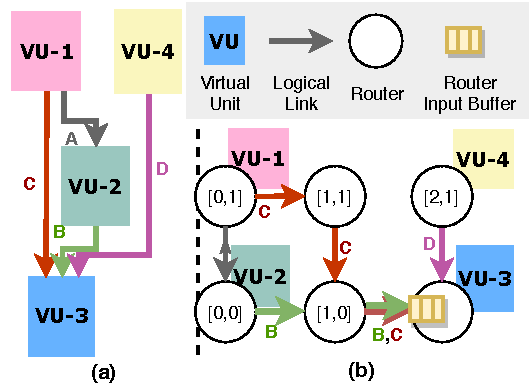
\includegraphics[width=0.5\columnwidth]{figs/deadlock.pdf}
  \caption{An example of deadlock in a streaming accelerator, showing the (a) VU data-flow graph and (b) physical placement and routes on a $2\times3$ network. There are input buffers at all router inputs, but only the buffer of interest is shown.}\small\textsuperscript{}\label{fig:deadlock}
\end{figure}

%Deadlock is a system pathology that occurs when multiple actors hold resources while waiting for each other's resources to become available.
%In a NoC, the actors are flits, and the held/waited-for resources are buffers.
%There are four necessary conditions for permament deadlock \cite{coffman1971system}:
%\begin{enumerate}
%  \item resources are mutually exclusive,
%  \item actors hold resources while waiting on other resources,
%  \item actors can not be preempted, and
%  \item actors wait on each other in a cyclic graph.
%\end{enumerate}

%In traditional NoC designs, there are two types of deadlock: deadlock within a network (such as that from cyclic paths), and \emph{protocol deadlock}.
%These designs are typically based around a request-response model: to avoid protocol deadlock, a node issuing a request will always be ready to receive its response. 
%Then, to ensure that the protocol graph is acyclic, the responses are prevented from waiting indefinitely on resources held by requests by partitioning all buffers in the network into two classes.
%Deadlock within a network is avoided by a variety of schemes, many of which (dateline VC allocation, dimension-order routing) work by imposing restrictions on which holds/waits relationships are valid.
%These restrictions ensure that the full potential holds/waits graph is acyclic, and therefore any subgraph must also be acyclic.

%When extending the deadlock model to a CGRA, there are three main types of deadlock that we need to avoid: traditional network deadlock, endpoint buffer deadlock, and through-node deadlock.
%For CGRAs, there are three main types of deadlock that we need to avoid: traditional network deadlock, endpoint buffer deadlock, and through-node deadlock.
%The key difference between CGRA and CPU networks is that CGRAs operate in a streaming fashion---each spatially distributed node, after completing its assigned work, sends the result to the next node(s).
%Furthermore, each node has fixed-size input buffers which, with the long distances possible between nodes, are far too small to perform high-throughput end to end credit-based flow control \cite{wang2013avoiding}.
%Finally, nodes propagate backpressure signals from their outputs to their inputs, which means that they must be considered as part of the network graph \cite{hansson2007avoiding}.
%This is similar to work done on streaming NoCs, where multiple streams of traffic compete for the same resources \cite{hansson2007avoiding, wang2013avoiding}.
%\begin{figure}
  %\centering
  %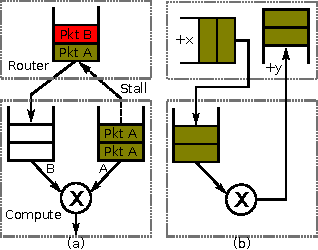
\includegraphics[width=0.4\columnwidth]{figs/deadlock_figs.pdf}
  %\caption{Two forms of network deadlock for CGRA dynamic networks. The left shows input buffer starvation, and the right shows a packet taking an ``illegal'' turn through a node.}
  %\label{fig:deadlock}
%\end{figure}
%Furthermore, because a compute node must be able to send its output to read its inputs, dependences may be propagated backwards through the network; this means that dimension order routing alone is insufficient to make progress and separate virtual networks must be used.
%\subsection{Endpoint Buffer Deadlock}
%This is a type of protocol deadlock that results from head-of-line blocking and finite buffer sizes at node inputs, as shown in Figure~\ref{fig:deadlock}(a).
%Consider two streams, A and B, that traverse the same virtual channel but are destined for different input buffers at the same destination node.
%If A fills up its input buffer, and B's input buffer is empty, the node cannot make progress.
%Simultaneously, if a flit from stream A is at the head of the shared virtual channel, then no flits from stream B will be able to pass it.
%
%At the final hop of the network, this would be trivial to resolve: the final router can use its knowledge of the buffer state of the destination to avoid overloading any single input buffer.
%However, it could be too late to resolve this problem at the final router, because if it blocks the faster flow, and they share a network resource earlier, the slower flow could be head-of-line blocked earlier in the network.
%\subsection{Through-Node Deadlock}
%Because nodes do not have infinite buffers, the deadlock graph for a network no longer begins and ends at the routes---it must be extended with information about the program nodes \cite{hansson2007avoiding}.
%%This means that traditional deadlock avoidance techniques, such as dimension-order routing, are \emph{not sufficient} to prevent deadlock in these networks.
%An example of how this can cause deadlock in a y-first dimension-order routed network is shown in Figure~\ref{fig:deadlock}(b).
%This type of deadlock can also combine with endpoint deadlock, in addition to traditional network deadlock.
%Because nodes propagate holds/waits dependences, any indirect input to the final node is capable of creating an endpoint buffer deadlock at the final node with any other indirect input, anywhere in the network.
%When different branches of the tree are fed by different DRAM accesses, one will almost certainly run faster and inevitably lead to this deadlock condition.
%Practically, this means that no two logical paths may be allowed to conflict at \emph{any} point in the network; to meet this guarantee, buffer allocation is performed to ensure that all logical paths traversing the same physical link are placed into separate virtual channels.
%Because there are only a finite number of VCs at each router, this is another network constraint to optimize: routes are penalized for exceeding the maximum, which leads to them being moved and a better solution being found.

\subsection{Heuristic Routing Guild Generation} \label{sec:heuristic}

In Spatial, the user can annotate runtime-variable input values to assist compiler analysis.  
We use these programmer annotations to compute the expected number of iterations for each controller statically; this heuristic guidance helps the placer evenly distribute traffic. 
However, we do not require exact annotations for efficient placement---a rough estimate of data size is sufficient for the placer to determine the relative importance of links.
For loop controllers, the number of iterations per parent iteration is $\lceil(max-min)/(step\cdot par)\rceil;$ controllers representing glue logic run once per parent iteration.
The activation count of a link will be the product of all of its ancestral controllers' iteration counts.
%Another controller in Spatial runs forever while there are elements in its streaming input buffers. 
%This construct is analogous to while loop condition on FIFO emptyness in software programming model. 
%For these, we allow the user to annotate the number of elements coming from the streaming input, and the compiler can derive the activion count of other controllers relative to the streaming controller.

%The relative enqueue and dequeue rate of each memory relative to its producer and consumer controllers can be computed based on source of the control signal, which usually is the enable or done signal of a counter in the controller branch. 
%For example, for register \emph{N} in \emph{VU-D}, it is enqueued every cycle when producer \emph{C0-1} is enabled and dequeued every time \emph{C1.done} is high. 
%Then enqueue rate of register \emph{N} is just 1, while the dequeue rate of \emph{N} is the product if iteration counts of \emph{C4-1}, \emph{C4}, \emph{C3}, and \emph{C1} $\left(\frac{N^2}{tsA \cdot ip \cdot op2 \cdot op1}\right)$.
%For any link $L$, the total number of active cycles can be computed as activation of its producer devided by the enqueue rate.
%In absence of streaming controllers, the total number of activation of a controller is just a product of itself and its ancestors's iteration counts. In case of streamiing controller, the number of activation is the links's activation count multiplied by the enqueuing rate.

%Once we know the number of times each link is activated in the application, the placer can prioritize using static network to route links that carry high activation counts to guarantee throughput requirement of the data flow pipeline, and encourage link sharing across virtual links with low activations count without harming the performance. 
Using the computed activation counts, the placer prioritizes highly used links for allocation to the static network and leaves infrequently used links on the dynamic network. 
When no annotation is provided, or loop bounds cannot be constant-propagated, the compiler estimates loop iteration counts based on the nesting depth: innermost loops are the most frequently active.
This heuristic provides a reasonable estimate of links' priorities for routing purposes.
